% Emacs settings: -*-mode: latex; TeX-master: "manual.tex"; -*-

\section{Single\_crystal: The single crystal component}
\label{s:Single_crystal}
\index{Samples!Single crystal diffraction}
\index{Diffraction}
\index{Incoherent elastic scattering}

\subsection{The physical model}

The textbook expression for the scattering cross-section of a crystal
is~\cite{squires}:
$$
\left(\frac{d\sigma}{d\Omega}\right)_{\rm coh.el.} =
        N\frac{(2\pi)^3}{V_0}\sum_{\boldsymbol{\tau}}
        \delta(\boldsymbol{\tau} - \boldsymbol{\kappa})|F_{\boldsymbol{\tau}}|^2
$$
Here $|F_{\boldsymbol{\tau}}|^2$ is the structure factor, $N$ is the
number of unit cells, $V_0$ is the volume of an
individual unit cell, and $\boldsymbol{\kappa} = {\bf k}_i - {\bf
  k}_f$ is the scattering vector. $\delta(\boldsymbol{x})$ is a 3-dimensional delta
function in reciprocal space,
so for given incoming wave vector ${\bf k}_i$ and lattice vector
${\boldsymbol{\tau}}$, only a single final wave vector ${\bf k}_f$ is allowed.
In a real crystal, however, reflections are not perfectly sharp. Because
of imperfection and finite-size effects, there will be a small region
around $\boldsymbol{\tau}$ in reciprocal space of possible scattering vectors.

The Single\_crystal component simulates a crystal with a mosaic spread
$\eta$ and a lattice plane spacing uncertainty $\Delta d/d$. In such
crystals the reflections will not be completely sharp;
there will be a small region around each reciprocal lattice point of the
crystal that contains valid scattering vectors.

We model the mosaicity and $\Delta d/d$ of the crystal with
3-dimensional Gaussian functions in reciprocal space (see
figure~\ref{fig:crystal-reciprocal-space}). Two of the axes of the
Gaussian are perpendicular to the reciprocal lattice vector $\boldsymbol{\tau}$ and model
the mosaicity. The third one is parallel to $\boldsymbol{\tau}$ and models
$\Delta d/d$. We assume that the
mosaicity is small so that the possible directions of the scattering
vector may be approximated with a Gaussian in rectangular
coordinates.
\begin{figure}[t]
  \begin{center}
    \psfrag{ki}[r][r]{$\boldsymbol{k}_{\rm i}$}
    \psfrag{kf}[l][l]{$\boldsymbol{k}_{\rm f}$}
    \psfrag{tau}[r][r]{$\boldsymbol{\tau}$}
    \psfrag{mosaic}[l][l]{$\eta$}
    \psfrag{del-d-d}[l][l]{$\Delta d/d$}
    \psfrag{Ewald}[l][l]{Ewald}
    \psfrag{Sphere}[l][l]{Sphere}
    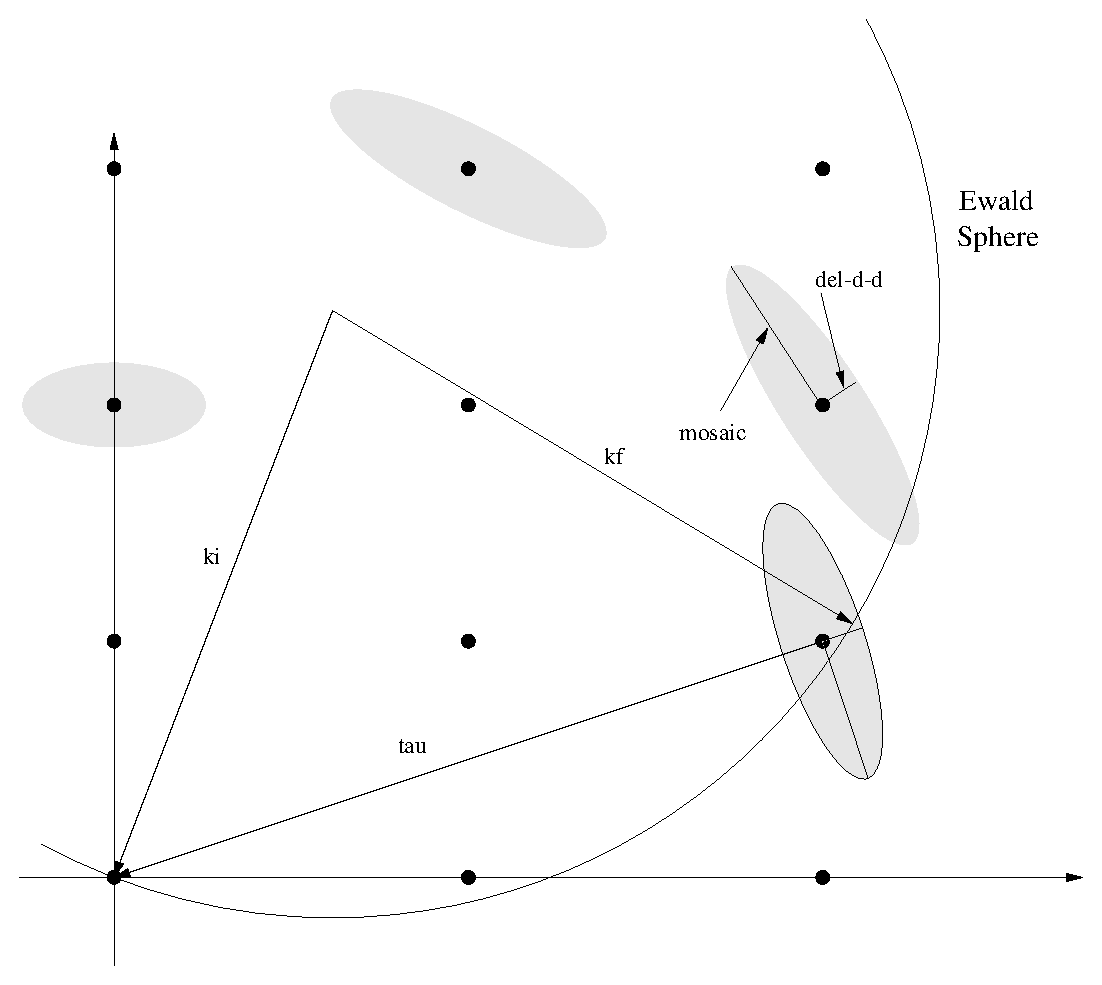
\includegraphics[width=0.7\textwidth]{figures/recip_space3.eps}
  \end{center}
\caption{Ewald sphere construction for a single neutron showing the
    Gaussian broadening of reciprocal lattice points in their local
    coordinate system.}
\label{fig:crystal-reciprocal-space}
\end{figure}

If the mosaic is isotropic (the same in all directions), the two
Gaussian axes perpendicular to $\boldsymbol{\tau}$ are simply arbitrary
normal vectors of equal length given by the mosaic. But if the mosaic
is anisotropic, the two perpendicular axes will in general be different
for each scattering vector. In the absence of anything better, the
Single\_crystal component uses a model which is at least mathematically
plausible and which works as expected in the two common cases:
(1)~isotropic mosaic, and (2)~two mosaic directions (``horizontal and
vertical mosaic'') perpendicular to a scattering vector.

The basis for the model is a three-dimensional Gaussian distribution in
Euler angles giving the orientation probability distribution for the
micro-crystals; that is, the misorientation is given by small rotations
around the $X$, $Y$, and $Z$ axes, with the rotation angles having (in
general different) Gaussian probability distributions. For given
scattering vector $\boldsymbol{\tau}$, a rotation of the micro-crystals
around an axis parallel to $\boldsymbol{\tau}$ has no effect on the
direction of the scattering vector. Suppose we form the intersection
between the three-dimensional Gaussian in Euler angles and a plane
through the origin perpendicular to $\boldsymbol{\tau}$. This gives a
two-dimensional Gaussian, say with axes defined by unit vectors
$\boldsymbol{g}_1$ and $\boldsymbol{g}_2$ and mosaic widths $\eta_1$ and
$\eta_2$.

We now let the mosaic for $\boldsymbol{\tau}$ be defined by rotations
around $\boldsymbol{g}_1$ and $\boldsymbol{g}_2$ with angles having
Gaussian distributions of widths $\eta_1$ and $\eta_2$. Since
$\boldsymbol{g}_1$, $\boldsymbol{g}_2$, and $\boldsymbol{\tau}$ are
perpendicular, a small rotation of $\boldsymbol{\tau}$ around
$\boldsymbol{g}_1$ will change $\boldsymbol{\tau}$ in the direction of
$\boldsymbol{g}_2$. The two axes of the Gaussian mosaic in reciprocal
space that are perpendicular to $\boldsymbol{\tau}$ will thus be given
by $\tau\eta_2\boldsymbol{g}_1$ and $\tau\eta_1\boldsymbol{g}_2$.

We now derive a quantitative expression for the scattering cross-section
of the crystal in the model. For this, we introduce a \emph{local
  coordinate system} for each reciprocal lattice point
$\boldsymbol{\tau}$ and use $\boldsymbol{x}$ for vectors written in local
coordinates. The origin is $\boldsymbol{\tau}$, the first axis
is parallel to $\boldsymbol{\tau}$ and the other two axes are
perpendicular to $\boldsymbol{\tau}$. In the local coordinate system,
the 3-dimensional Gaussian is given by
\begin{equation}
  \label{eq:crystal-gauss-1}
  G(x_1,x_2,x_3) = \frac{1}{(\sqrt{2\pi})^3}\frac{1}{\sigma_1\sigma_2\sigma_3}
  e^{-\frac{1}{2}(\frac{x_1^2}{\sigma_1^2} +
  \frac{x_2^2}{\sigma_2^2} + \frac{x_3^2}{\sigma_3^2})}
\end{equation}
The axes of the Gaussian are $\sigma_1 = \tau\Delta d/d$ and $\sigma_2 =
\sigma_3 = \eta\tau$. Here we used the assumption that $\eta$ is small,
so that $\tan\eta \approx \eta$ (with $\eta$ given in radians).  By
introducing the diagonal matrix
$$
D = \left(
  \begin{array}[c]{ccc}
    \frac{1}{2}\sigma_1^2 & 0 & 0 \\
    0 & \frac{1}{2}\sigma_2^2 & 0 \\
    0 & 0 & \frac{1}{2}\sigma_3^2
  \end{array}\right)
$$
equation~(\ref{eq:crystal-gauss-1}) can be written as
\begin{equation}
  G(\boldsymbol{x}) =
  \frac{1}{(\sqrt{2\pi})^3}\frac{1}{\sigma_1\sigma_2\sigma_3}
  e^{-\boldsymbol{x}^{\rm T} D \boldsymbol{x}}
\end{equation}
again with $\boldsymbol{x}=(x_1,x_2,x_3)$ written in local coordinates.

To get an expression in the coordinates of the reciprocal lattice of the
crystal, we introduce a matrix $U$ such that if $\boldsymbol{y} =
(y_1,y_2,y_3)$ are the global coordinates of a point in the crystal
reciprocal lattice, then $U(\boldsymbol{y} + \boldsymbol{\tau})$ are the
coordinates in the local coordinate system for $\boldsymbol{\tau}$. The
matrix $U$ is given by
$$ U^{\rm T} = (\hat{u}_1, \hat{u}_2, \hat{u}_3), $$
where $\hat{u}_1$, $\hat{u}_2$, and $\hat{u}_3$ are the axes of the
local coordinate system, written in the global coordinates of the
reciprocal lattice. Thus
$\hat{u}_1 = \boldsymbol{\tau}/\tau$,  and $\hat{u}_2$ and $\hat{u}_3$ are
unit vectors perpendicular to $\hat{u}_1$ and to each other.
The matrix $U$ is unitarian, that is
$U^{-1} = U^{\rm T}$. The translation between global and local
coordinates is
$$ \boldsymbol{x} = U(\boldsymbol{y} + \boldsymbol{\tau}) \qquad
   \boldsymbol{y} = U^{\rm T} \boldsymbol{x} - \boldsymbol{\tau} $$

The expression for the 3-dimensional Gaussian in global coordinates is
\begin{equation}
  G(\boldsymbol{y}) =
  \frac{1}{(\sqrt{2\pi})^3}\frac{1}{\sigma_1\sigma_2\sigma_3}
  e^{-(U(\boldsymbol{y}+\boldsymbol{\tau}))^{\rm T} D (U(\boldsymbol{y}+\boldsymbol{\tau}))}
\end{equation}
The elastic coherent cross-section is then given by
\begin{equation}
  \label{eq:crystal-cross-section}
  \left(\frac{d\sigma}{d\Omega}\right)_{\rm coh.el.} =
        N\frac{(2\pi)^3}{V_0}\sum_{\boldsymbol{\tau}}
        G(\boldsymbol{\tau} - \boldsymbol{\kappa})
         |F_{\boldsymbol{\tau}}|^2
\end{equation}

The user must specify a list of reciprocal lattice vectors
$\boldsymbol{\tau}$ to consider along with their structure factors
$|F_{\boldsymbol{\tau}}|^2$. The user must also specify the coordinates
(in direct space) of the unit cell axes $\boldsymbol{a}$,
$\boldsymbol{b}$, and $\boldsymbol{c}$, from which the reciprocal lattice
will be computed.

In addition to coherent scattering, the Single\_crystal component also
handles incoherent scattering amd absorption. The incoherent scattering
cross-section is supplied by the user as a constant $\sigma_{\rm
  inc}$. The absorption cross-section is supplied by the user at
2200~m/s, so the actual cross-section for a neutron of velocity $v$ is
$\sigma_{\rm abs} = \sigma_{2200} \frac{\rm 2200~m/s}{v}$.

\subsection{The algorithm}

The overview of the algorithm used in the Single\_crystal component is
as follows:
\begin{enumerate}
\item\label{enum:crystal-1} Check if the neutron intersects the
  crystal. If not, no action is taken.
\item\label{enum:crystal-2} Search through a list of reciprocal lattice
  points of interest, selecting those that are close enough to the Ewald
  sphere to have a non-vanishing scattering probability. From these,
  compute the total coherent cross-section $\sigma_{\rm coh}$ (see
  below), the absorption cross-section $\sigma_{\rm abs} = \sigma_{\rm
  2200} \frac{{\rm 2200~m/s}}{v}$, and the total cross-section
  $\sigma_{\rm tot} = \sigma_{\rm coh}+\sigma_{\rm inc}+\sigma_{\rm abs}$.
\item\label{enum:crystal-3} The transmission probability is
  $\exp(\frac{\sigma_{\rm tot}}{V_0}\ell)$ where $\ell$ is the length of
  the flight path through the crystal. A Monte Carlo choice is made
  whether the neutron is transmitted or not. Optionally, the user may
  set a fixed Monte Carlo probability for the first scattering event,
  for example to boost the statistics for a weak reflection.
\item\label{enum:crystal-4} For non-transmission, the position at which
  the neutron will interact is selected from an exponential
  distribution. A Monte Carlo choice is made of whether to scatter
  coherently or incoherently. Absorption is treated by weight adjustment
  (see below).
\item\label{enum:crystal-5} For incoherent scattering, the outgoing wave
  vector $\boldsymbol{k}_{\rm f}$ is selected with a random direction.
\item\label{enum:crystal-6} For coherent scattering, a reciprocal
  lattice vector is selected by Monte Carlo choice, and
  $\boldsymbol{k}_{\rm f}$ is found (see below).
\item\label{enum:crystal-7} Adjust the neutron weight as dictated by the
  Monte Carlo choices made.
\item\label{enum:crystal-8} Repeat from~(\ref{enum:crystal-2}) until the
  neutron is transmitted (to simulate multiple scattering).
\end{enumerate}

For point~\ref{enum:crystal-2}, the distance
\textit{dist} between a reciprocal lattice point and the Ewald sphere is
considered small enough to allow scattering if it is less than five
times the maximum axis of the Gaussian, $\textit{dist} \leq
5\max(\sigma_1,\sigma_2,\sigma_3)$.

\paragraph{Choosing the outgoing wave vector}

The final wave vector $\boldsymbol{k}_{\rm f}$ must lie on the
intersection between the Ewald sphere and the Gaussian ellipsoid. Since
$\eta$ and $\Delta d/d$ are assumed small, the intersection can be
approximated with a plane tangential to the sphere, see
figure~\ref{fig:crystal-scattering-tri}. The tangential point is taken
to lie on the line between the center of the Ewald sphere
$-\boldsymbol{k}_{\rm i}$ and the reciprocal lattice point
$\boldsymbol{\tau}$. Since the radius of the Ewald sphere is $k_{\rm
  i}$, this point is
$$ \boldsymbol{o}=(1 - k_{\rm i}/\rho)\boldsymbol{\rho} - \boldsymbol{\tau} $$
where $\rho = \boldsymbol{k}_{\rm i} - \boldsymbol{\tau}$.
\begin{figure}[t]
  \begin{center}
    \psfrag{ki}[r][r]{$\boldsymbol{k}_{\rm i}$}
    \psfrag{kf}[l][l]{$\boldsymbol{k}_{\rm f}$}
    \psfrag{rho}[r][r]{$\boldsymbol{\rho}$}
    \psfrag{tau}[r][r]{$\boldsymbol{\tau}$}
    \psfrag{x}[l][l]{$\boldsymbol{x}$}
    \psfrag{Ewald}[r][r]{Ewald}
    \psfrag{Sphere}[r][r]{Sphere}
    \psfrag{Tangential}[l][l]{Tangential}
    \psfrag{plane}[l][l]{plane}
    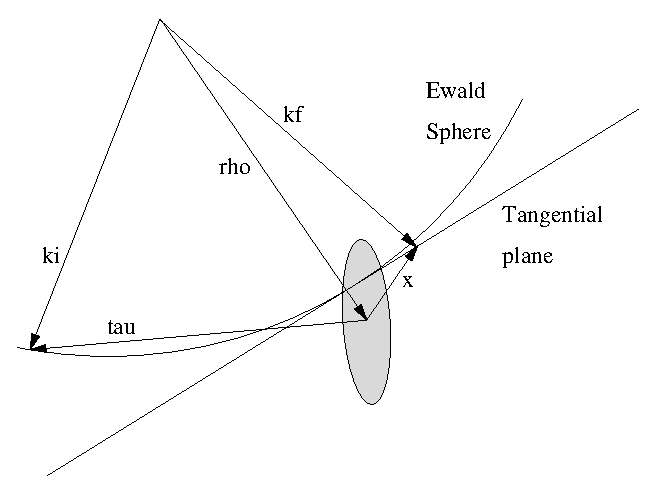
\includegraphics[width=0.7\textwidth]{figures/recip-detail.eps}
  \end{center}
\caption{The scattering triangle in the single crystal.}
\label{fig:crystal-scattering-tri}
\end{figure}

The equation for the plane is
\begin{equation}
  \label{eq:crystal-tangent-plane}
    \boldsymbol{P}(\boldsymbol{t}) = \boldsymbol{o} + B \boldsymbol{t}, \qquad
    \boldsymbol{t} \in \mathbb{R}^2
\end{equation}
Here $B = (\boldsymbol{b}_1, \boldsymbol{b}_2)$ is a $3\times 2$ matrix
with the two generators for the plane $\boldsymbol{b}_1$ and
$\boldsymbol{b}_2$. These are (arbitrary) unit vectors in the plane,
being perpendicular to
each other and to the plane normal $\boldsymbol{n} =
\boldsymbol{\rho}/\rho$.

Each $\boldsymbol{t}$ defines a potential final wave vector
$\boldsymbol{k}_{\rm f}(\boldsymbol{t}) = \boldsymbol{k}_{\rm i} +
\boldsymbol{P}(\boldsymbol{t})$. The value of the 3-dimensional Gaussian
for this $\boldsymbol{k}_{\rm f}$ is
\begin{equation}
  \label{eq:crystal-gauss-t-1}
  G(\boldsymbol{x}(\boldsymbol{t})) =
  \frac{1}{(\sqrt{2\pi})^3}\frac{1}{\sigma_1\sigma_2\sigma_3}
  e^{-\boldsymbol{x}(\boldsymbol{t})^{\rm T} D \boldsymbol{x}(\boldsymbol{t})}
\end{equation}
where $\boldsymbol{x}(\boldsymbol{t}) = \boldsymbol{\tau} -
(\boldsymbol{k}_{\rm i} - \boldsymbol{k}_{\rm f}(\boldsymbol{t}))$ is
given in local coordinates for $\boldsymbol{\tau}$. It can be shown that
equation~(\ref{eq:crystal-gauss-t-1}) can be re-written as
\begin{equation}
  \label{eq:crystal-gauss-2}
  G(\boldsymbol{x}(\boldsymbol{t})) =
  \frac{1}{(\sqrt{2\pi})^3}\frac{1}{\sigma_1\sigma_2\sigma_3} e^{-\alpha}
  e^{-(\boldsymbol{t}-\boldsymbol{t}_0)^{\rm T} M
    (\boldsymbol{t}-\boldsymbol{t}_0)}
\end{equation}
where $M = B^{\rm T} D B$ is a $2 \times 2$ symmetric and positive
definite matrix, $\boldsymbol{t}_0 = -M^{-1}B^{\rm T} D \boldsymbol{o}$
is a 2-vector, and $\alpha = -\boldsymbol{t}_0^{\rm T} M
\boldsymbol{t}_0 + \boldsymbol{o}^{\rm T} D \boldsymbol{o}$ is a real
number.  Note that this is a two-dimensional Gaussian (not necessarily
normalized) in $\boldsymbol{t}$ with center $\boldsymbol{t}_0$ and axis
defined by $M$.

To choose $\boldsymbol{k}_{\rm f}$ we sample $\boldsymbol{t}$ from the
2-dimensional Gaussian distribution~(\ref{eq:crystal-gauss-2}). To do
this, we first construct the Cholesky decomposition of the matrix
$(\frac{1}{2}M^{-1})$. This gives a $2\times 2$ matrix $L$ such that $L
L^{\rm T} = \frac{1}{2}M^{-1}$ and is possible since $M$ is symmetric
and positive definite. It is given by
$$
  L = \left(
  \begin{array}[c]{cc}
    \sqrt{\nu_{11}} & 0 \\
    \frac{\nu_{12}}{\sqrt{\nu_{11}}} & \sqrt{\nu_{22} - \frac{\nu_{12}^2}{\nu_{11}}}
  \end{array}\right)
\qquad\hbox{where }
  \frac{1}{2}M^{-1} = \left(
  \begin{array}[c]{cc}
    \nu_{11} & \nu_{12} \\
    \nu_{12} & \nu_{22}
  \end{array}\right)
$$
Now let $\boldsymbol{g} = (g_1, g_2)$ be two random numbers drawn form a
Gaussian distribution with mean 0 and standard deviation 1, and let
$\boldsymbol{t} = L\boldsymbol{g} + \boldsymbol{t}_0$. The probability
of a particular $\boldsymbol{t}$ is then
\begin{eqnarray}
  P(\boldsymbol{t})d\boldsymbol{t}
    &=& \frac{1}{2\pi}
      e^{-\frac{1}{2}\boldsymbol{g}^{\rm T}\boldsymbol{g}} d\boldsymbol{g} \\
    &=& \frac{1}{2\pi}\frac{1}{\det L}
      e^{-\frac{1}{2}(L^{-1}(\boldsymbol{t}-\boldsymbol{t}_0))^{\rm T}
          (L^{-1}(\boldsymbol{t}-\boldsymbol{t}_0))} d\boldsymbol{t} \\
    &=& \frac{1}{2\pi}\frac{1}{\det L}
      e^{-(\boldsymbol{t}-\boldsymbol{t}_0)^{\rm T}
          M(\boldsymbol{t}-\boldsymbol{t}_0)} d\boldsymbol{t}
  \label{eq:crystal-gauss-prob-1}
\end{eqnarray}
where we used that
$\boldsymbol{g}=L^{-1}(\boldsymbol{t}-\boldsymbol{t}_0)$ so that
$d\boldsymbol{g} = \frac{1}{\det L}d\boldsymbol{t}$. This is just the
normalized form of~(\ref{eq:crystal-gauss-2}). Finally we set
$\boldsymbol{k}'_{\rm f} = \boldsymbol{k}_{\rm i} +
\boldsymbol{P}(\boldsymbol{t})$ and
$\boldsymbol{k}_{\rm f} = (k_{\rm i}/k'_f)\boldsymbol{k}'_{\rm f}$ to
normalize the length of $\boldsymbol{k}_{\rm f}$ to correct for the
(small) error introduced by approximating the Ewald sphere with a plane.

\paragraph{Computing the total coherent cross-section}

To get the total coherent scattering cross-section, the differential
cross-section must be integrated over the Ewald sphere:
$$
\sigma_{\rm coh} = \int_{\rm Ewald}
\left(\frac{d\sigma}{d\Omega}\right)_{\rm coh.el.} d\Omega
$$
For small mosaic we may approximate the sphere with the tangential
plane, and we thus get from~(\ref{eq:crystal-cross-section})
and~(\ref{eq:crystal-gauss-2}):
\begin{eqnarray}
  \label{eq:crystal-coh-cs}
  \sigma_{{\rm coh},\boldsymbol{\tau}} &=& \int N\frac{(2\pi)^3}{V_0}
        G(\boldsymbol{\tau} - \boldsymbol{\kappa})
         |F_{\boldsymbol{\tau}}|^2 d\Omega \\
  &=& \frac{1}{\boldsymbol{k}_i^2} N\frac{(2\pi)^3}{V_0}
         \frac{1}{(\sqrt{2\pi})^3}\frac{e^{-\alpha}}{\sigma_1\sigma_2\sigma_3}
         |F_{\boldsymbol{\tau}}|^2
         \int e^{-(\boldsymbol{t}-\boldsymbol{t}_0)^{\rm T} M
         (\boldsymbol{t}-\boldsymbol{t}_0)}
         d\boldsymbol{t} \\
  &=& \det(L) \frac{1}{\boldsymbol{k}_i^2} N\frac{(2\pi)^{3/2}}{V_0}
         \frac{e^{-\alpha}}{\sigma_1\sigma_2\sigma_3}
         |F_{\boldsymbol{\tau}}|^2
         \int e^{-\frac{1}{2}\boldsymbol{g}^{\rm T}\boldsymbol{g}}
         d\boldsymbol{g} \\
  &=& 2\pi\det(L) \frac{1}{\boldsymbol{k}_i^2} N\frac{(2\pi)^{3/2}}{V_0}
         \frac{e^{-\alpha}}{\sigma_1\sigma_2\sigma_3}
         |F_{\boldsymbol{\tau}}|^2 \\
  &=& \frac{\det(L)}{\boldsymbol{k}_i^2} N\frac{(2\pi)^{5/2}}{V_0}
         \frac{e^{-\alpha}}{\sigma_1\sigma_2\sigma_3}
         |F_{\boldsymbol{\tau}}|^2 \\
  \sigma_{\rm coh} &=& \sum_{\boldsymbol{\tau}} \sigma_{{\rm coh},\boldsymbol{\tau}}
\end{eqnarray}
As before, we let $\boldsymbol{g} = L^{-1}(\boldsymbol{t} -
\boldsymbol{t}_0)$ so that $d\boldsymbol{t} = \det(L) d\boldsymbol{g}$.

\paragraph{Adjusting the neutron weight}

We now calculate the correct neutron weight adjustment for the Monte
Carlo choices made. In three cases is a Monte Carlo choice made with a
probability different from the probability of the corresponding physical
event: When deciding whether to transmit the neutron or not, when
simulating absorption, and when selecting the reciprocal lattice vector
$\boldsymbol{\tau}$ to scatter from.

If the user has choosen a fixed transmission probability $f({\rm
  transmit}) = p_{\rm transmit}$, the neutron weight must be adjusted by
$$ \pi({\rm transmit}) = \frac{\Pi({\rm transmit})}{f({\rm transmit})}
$$
where $\Pi({\rm transmit}) = \exp(\frac{\sigma_{\rm tot}}{V_0}\ell)$ is
the physical transmission probability. Likewise, for non-transmission
the adjustment is
$$ \pi({\rm no~transmission}) = \frac{1-\Pi({\rm transmit})}{1-f({\rm transmit})}.
$$

Absorption is never explicitly simulated, so the Monte Carlo probability
of coherent or incoherent scattering is $f({\rm coh}|{\rm inc}) =
1$. The physical probability of coherent or incoherent scattering is
$$ \Pi({\rm coh}|{\rm inc}) = \frac{\sigma_{\rm coh} + \sigma_{\rm
    inc}}{\sigma_{\rm tot}}, $$
so again a weight adjustment $\pi({\rm coh}|{\rm inc}) = \Pi({\rm
    coh}|{\rm inc})/f({\rm coh}|{\rm inc})$ is needed.

When choosing the reciprocal lattice vector $\boldsymbol{\tau}$ to
scatter from, the relative probability for $\boldsymbol{\tau}$ is
$r_{\boldsymbol{\tau}} = \sigma_{{\rm
    coh},\boldsymbol{\tau}}/|F_{\boldsymbol{\tau}}|^2$. This is done to
get better statistics for weak reflections. The Monte Carlo probability
for the reciprocal lattice vector $\boldsymbol{\tau}$ is thus
$$ f(\boldsymbol{\tau}) =
\frac{r_{\boldsymbol{\tau}}}{\sum_{\boldsymbol{\tau}} r_{\boldsymbol{\tau}}}
$$
whereas the physical probability is $\Pi(\boldsymbol{\tau}) = \sigma_{{\rm
    coh},\boldsymbol{\tau}}/\sigma_{\rm coh}$. A weight adjustment is
thus needed of
$$
\pi(\boldsymbol{\tau}) =
 \frac{\Pi(\boldsymbol{\tau})}{f(\boldsymbol{\tau})} =
 \frac{\sigma_{{\rm coh},\boldsymbol{\tau}}
  \sum_{\boldsymbol{\tau}} r_{\boldsymbol{\tau}}}{\sigma_{\rm coh}
  r_{\boldsymbol{\tau}}}.$$

\subsection{The implementation}

The equations describing the Single\_crystal simulation are quite
complex, and consequently the code is fairly sizeable. Most of it is
just the expansion of the vector and matrix equations in individual
coordinates, and should thus be straightforward to follow.

The implementation pre-computes a lot of the necessary values in the
\texttt{INITIALIZE} section. It is thus actually very efficient despite
the complexity. If the list of reciprocal lattice points is big,
however, the search through the list will be slow. The precomputed data
is stored in the structures \texttt{hkl\_info} and in an array of
\texttt{hkl\_data} structures (one for each reciprocal lattice point in
the list). In addition, for every neutron event an array of
\texttt{tau\_data} is computed with one element for each reciprocal
lattice point close to the Ewald sphere. Except for the search for
possible $\boldsymbol{\tau}$ vectors, all computations are done in local
coordinates using the matrix $U$ to do the necessary transformations.

The list of reciprocal lattice points is specified in an ASCII data
file. Each line contains seven numbers, separated by white space. The
first three numbers are the $(h,k,l)$ indices of the reciprocal lattice
point, and the last number is the value of the structure factor
$|F_{\boldsymbol{\tau}}|^2$, in barns. The middle three numbers are not
used; they are nevertheless required since this makes the file format
compatible with the output from the Crystallographica
program~\cite{crystallographica}.

The input parameters for the component are \textit{xwidth},
\textit{yheight}, and \textit{zthick} to define the dimensions of the
crystal in meters; \textit{delta\_d\_d} to give the
value of $\Delta d/d$ (no unit);
$(\textit{ax}, \textit{ay}, \textit{az})$, $(\textit{bx}, \textit{by},
\textit{bz})$, and $(\textit{cx}, \textit{cy}, \textit{cz})$ to define
the axes of the direct lattice of the crystal (the sides of the unit
cell) in units of {\AA}ngstr{\o}m; and \textit{reflections}, a string
giving the name of the file with the list of structure factors to
consider. The mosaic is specified \emph{either} isotropically as
\textit{mosaic}, \emph{or} anisotropically as \textit{mosaic\_h}
(rotation around the $Y$ axis), \textit{mosaic\_v} (rotation around the
$Z$ axis), and \textit{mosaic\_n} (rotation around the $X$ axis); in all
cases in units of full-width-half-maximum minutes of arc.

Optionally, the absorption cross-section at 2200 m/s and the incoherent
cross-section may be given as \textit{absorbtion} and
\textit{incoherent} (in barns), with default of zero; and
\textit{p\_transmit} may be assigned a fixed Monte Carlo probability for
transmission through the crystal without any interaction.
